\part{Vorwort von Olaf Radicke}


\begin{floatingfigure}[l]{0.33\textwidth}
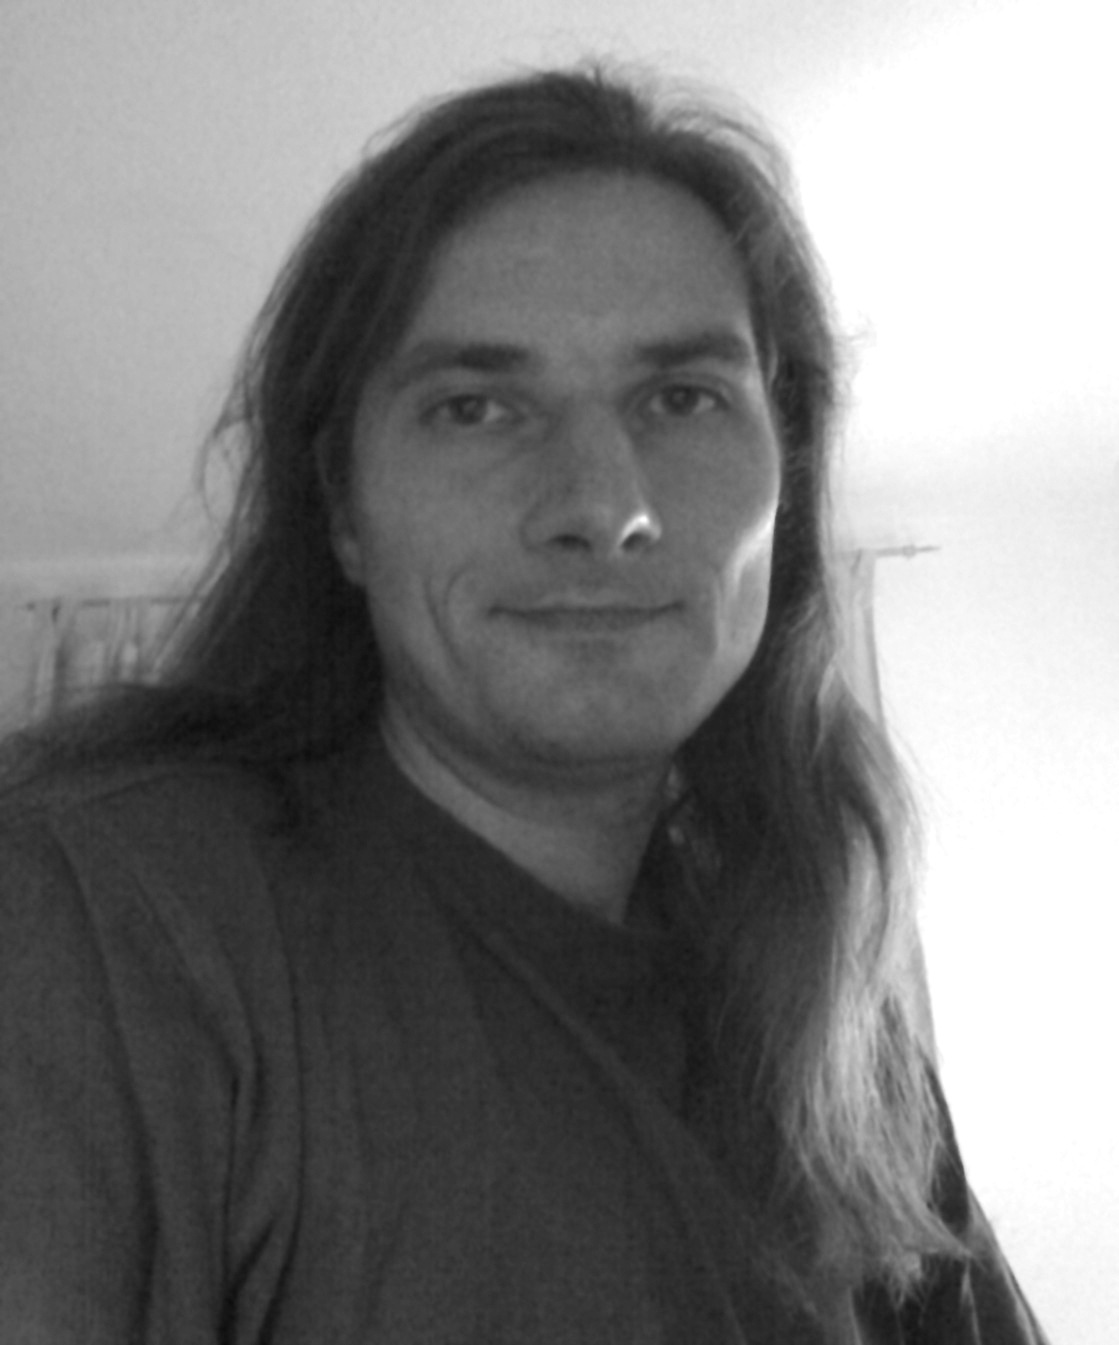
\includegraphics[width=0.33\textwidth]{olaf_radicke_bw}
\end{floatingfigure}

Ich habe ein sehr emotionale Beziehung zu dem Text. Ich hatte das Buch zufällig
entdeckt. Ich war für einige Monate in Nord-Thailand, um in buddhistischen
Klöstern zu meditieren. Zu diesem Zeitpunkt hatte ich mich 10 Jahre intensiv mit
Buddhismus beschäftigt und stellte fest, daß ich mit den buddhistischen Übungen
nicht weiter kam. Zu diesem Zeitpunkt liefen mir ein paar enthusiastische
Mitglieder der charismatischen Gemeinde \textit{"`Hope of Chiang Mai"'} über
den Weg. Sie bemühten sich redlich um meine Missionierung und luden mich zu
ihren \textit{Bibelkonkress} ein. Da ich die Leute ganz kauzig fand, ging ich
mit und dort fand ich auf dem (obligatorischen) Büchertisch eine Ausgabe
von \textit{"`no cross no crown"'}.
Ich konnte von dem Englisch kaum was verstehen, aber es sprach mich dermaßen
an, daß ich es kaufte. Die enttäuschte Reaktion meiner charismatischen Freunde,
als ich ihnen stolz meine Neuerwerbung präsentierte, bestärkte mich in meinem
Interesse an dem Buch. Der entscheidende Satz daraus, den ich gelesen und
verstanden hatte, war:

\begin{center}
\parbox{7,5cm}{
\textit{"`And as long as this disease continueth upon man he will make his God
his enemy, and himself incapable of the love and salvation that He hath
manifested, by his Son Jesus Christ, to the world."'}

\medskip

\textit{"`Als wenn er bloss um seiner selbst willen da sei, oder als ob er
sich selbst das Dasein gegeben habe, und daher keiner höheren Macht Rechenschaft
schuldig ist, und ihrem Urteilsspruch auch nicht unterworfen ist."'}
}
\end{center}

\medskip

Es dauerte noch eine Weile bis ich dann auf Quaker stieß und die deutsche
Übersetzung von \textit{"`no cross no crown"'}. Aber im Grunde wahr es ein
Bekehrungserlebnis. Ziemlich unspektakulär und nicht wirklich ein Bruch zum
Buddhismus. Es gibt viele Überschneidungen zwischen Buddhismus und Quakertum.
Ich denke, daß sich das Quakertum, besser als Buddhismus, in die westliche Welt (und das westliche
Denken) einpasst. Buddhismus vs. Quakertum ist aber noch mal
ein anderes Thema, was bestimmt auch sehr interessant ist, aber hier den Rahmen
sprengen würde.

\medskip

Claus Bernet hatte ich immer wieder von dem Buch erzählt. Irgendwann hat er mir
bei seinen Archiv-Recherchen das erste Kapitel der deutschen Übersetzung als
Fotokopie geschickt. Ich war aber sofort \textit{Feuer und
Flamme}. Ich ließ mir das gesamte Buch von ihm als Kopie schicken. Nach 1/3 war
ich davon überzeugt, daß der Text unbedingt wieder allgemein zugänglich und
bekannt gemacht werden sollte.

\medskip

Ich begann in dem Internet-Projekt \textit{de.WikiSource.org} von meinen Plänen
zu schreiben. Ich ließ dann für knapp 100 Euro vom Göttinger
Digitalisierungszentrum das Werk hochwertig einscannen. Das Ergebnis ist hier zu
finden:

\begin{center}
\texttt{http://gdz.sub.uni-goettingen.de/dms/load/img/?IDDOC=402779}
\end{center}

Danach wurde mir von Mitarbeitern des WikiSource-Projekts geholfen,
Texterkennungssoftware über die Scanns laufen zu lassen. Da es sich um
Altdeutsche Schrift handelt, wo das "`f"' und das "`s"' fast gleich aussieht,
und das "`b"' fast wie das "`d"', war das Ergebnis sehr fehlerhaft. In
zweimonatiger Arbeit, habe ich dann die Texte korrigiert und die Fussnoten
übertragen.

\medskip

Im nächsten Schritt habe ich dann den Text zu \LaTeX{} konvertiert und das Index
aufgebaut. In der Zwischenzeit konnte ich Claus Bernet von meinen Vorhaben überzeugen eine
Neuauflage herauszubringen. So stieg er dann mit ein und begann
den Text auf heutige Rechtschreibung anzupassen und einige der Texte zu
zusteuern, die die Erschliessung des Werkes von W. Penn erleichtern sollen.
Das Ergebnis ist nun das, welches jetzt vorliegt. Ich habe mir bewusst die
Option für weiter Auflagen offen gehalten, indem ich der Auflage die
\textit{Versionsnummer 1.0} gab. Ich würde mich über Rückmeldungen des Lesers
sehr freuen. Am besten bin ich unter der folgenden E-Mail-Adresse zu erreichen:

\begin{center}
\texttt{briefkasten@olaf-radicke.de}
\end{center}

Vielleicht noch kurz zu meiner Person: Ich bin 1971 in West-Berlin
\textit{Insulaner} geboren und protestantisch erzogen worden. Zunächst lernte
ich den Beruf des \textit{Schauwerbegestalters} indem ich aber nie gearbeitet
habe. Darauf folgten verschiedenste Jobs, immer wieder unterbrochen durch Zeiten
der Arbeitslosigkeit. In den letzten zehn Jahren habe ich zumeist in meinem
zweiten Beruf als Heilerziehungspfleger in der Behinderten-Assistenz gearbeitet.
Ich wohne in München und gehöre dort einer Gruppe Quaker an, die nicht zum
Verein \textit{Deutsche Jahresversammlung e.V}. gehört. Zu finden unter:

\begin{center}
\texttt{www.WasKannstDuSelbstSagen.de}
\end{center}

Und meinen privaten Weblog findet man unter:

\begin{center}
\texttt{www.Olaf-Radicke.de}
\end{center}

Zum Schluss bleibt mir nur zu wünschen, daß die hoffentlich zahlreichen Leser
den gleichen Gewinn aus dem Text ziehen, wie ich.


